% Latex template: mahmoud.s.fahmy@students.kasralainy.edu.eg
% For more details: https://www.sharelatex.com/learn/Beamer

\documentclass{beamer}					% Document class

\setbeamertemplate{footline}[text line]{%
  \parbox{\linewidth}{\vspace*{-8pt}Statistical Methods For Stochastic Biological Systems\hfill\insertshortauthor\hfill\insertpagenumber}}
\setbeamertemplate{navigation symbols}{}

\usepackage[english]{babel}				% Set language
\usepackage[utf8x]{inputenc}			% Set encoding

\mode<presentation>						% Set options
{
  \usetheme{default}					% Set theme
  \usecolortheme{default} 				% Set colors
  \usefonttheme{default}  				% Set font theme
  \setbeamertemplate{caption}[numbered]	% Set caption to be numbered
}

% Uncomment this to have the outline at the beginning of each section highlighted.
%\AtBeginSection[]
%{
%  \begin{frame}{Outline}
%    \tableofcontents[currentsection]
%  \end{frame}
%}

\usepackage{graphicx}					% For including figures
\usepackage{booktabs}					% For table rules
\usepackage{hyperref}					% For cross-referencing

\title{Deep generative models for biologists}	% Presentation title
\author{Clayton W. Seitz}								% Presentation author
\date{\today}									% Today's date	

\begin{document}

% Title page
% This page includes the informations defined earlier including title, author/s, affiliation/s and the date
\begin{frame}
  \titlepage
\end{frame}

% Outline
% This page includes the outline (Table of content) of the presentation. All sections and subsections will appear in the outline by default.
\begin{frame}{Outline}
  \tableofcontents
\end{frame}

% The following is the most frequently used slide types in beamer
% The slide structure is as follows:
%
%\begin{frame}{<slide-title>}
%	<content>
%\end{frame}


\section{Generative Models}

\begin{frame}{The logic of generative modeling}

Say we have a set of variables $\mathbf{x} = (x_{1},x_{2},...,x_{n})$ which might have some statistical dependence\\
\vspace{0.1in}
The variable $\mathbf{x}$ might be an amino acid sequence, DNA sequence, microscopy image, etc.\\
\vspace{0.1in}
\begin{itemize}
\item Often we are handed a batch of empirical samples $\{\mathbf{x}_{i}\}_{i=1}^{N}$
\item We want to know the generating distribution $p(\mathbf{x})$
\end{itemize}

In supervised \textcolor{red}{generative learning}, we try to explicity learn the joint distribution $p(\mathbf{x})=p(x_{1}|x_{2},...,x_{n})p(x_{2}|x_{3},...,x_{n}),...,p(x_{n})$, which is generally more difficult than discriminative learning. 

\end{frame}

\begin{frame}{Sampling from a model}

To find $p(\mathbf{x})$ we might fit a parametric model with parameters $\theta$ with MLE or some other method\\
\vspace{0.1in}
Lets assume we already know the model type and parameters $\theta$\\
\vspace{0.2in}
As a toy example, perhaps $x\sim \mathcal{N}(\mu,\sigma^{2})$ and we know $\theta = (\mu,\sigma)$\\
\vspace{0.1in}
In this simple case, we can draw samples by \textcolor{red}{rejection sampling}
\end{frame}

\begin{frame}{Rejection sampling with the uniform distribution}

Let $\Omega$ be the state space or \emph{support} of $x$. Let $U(\Omega)$ be the uniform distribution over $\Omega$\\
\vspace{0.1in}
Also notice that $p(x) \leq 1 \;\;\forall x \in \Omega$\\
\vspace{0.1in}
The following procedure produces a sample $x\sim p(x)$.
\begin{enumerate}
\item Sample $u\sim U(\Omega)$
\item Sample $y\sim U([0,1])$
\item If $y < p(u)$ return $y$ as a sample of $p(x)$
\end{enumerate}
\vspace{0.2in}
This algorithm suffers from the \textcolor{red}{curse of dimensionality}. Generally, sampling becomes 
\end{frame}

\begin{frame}{The sampling problem}

Dimensionality can make it difficult to sample from $p(\mathbf{x})$ directly. For example, the multivariate Gaussian distribution\\

\begin{equation*}
p(\mathbf{x}) = \frac{1}{(2\pi)^{n}|\Sigma|}\exp\left(-\frac{1}{2}(\mathbf{x}-\mu)^{T}\Sigma^{-1}(\mathbf{x}-\mu)\right)
\end{equation*}

Sampling must be achieved in another way e.g., \textcolor{red}{Cholesky decomposition} or \textcolor{red}{Gibbs sampling}


\end{frame}

\begin{frame}{The sampling problem}

We also may not know the proper normalization constant or \textcolor{red}{partition function} $Z$. Say we have

\begin{equation*}
p(\mathbf{x}) = \frac{1}{Z}\tilde{p}(\mathbf{x})
\end{equation*}

where $p(\mathbf{x})$ is easy to compute but $Z$ is (too) hard to compute.\\
\vspace{0.1in}
This \textcolor{red}{very important} situation arises in several contexts:\\
\vspace{0.1in}
1. In \textcolor{red}{Bayesian models} where $p(x_{1},x_{2}) := p(x_{1}|x_{2})p(x_{2})$ is easy to compute but
$Z = \int p(x_{1}|x_{2})p(x_{2})dx_{2}$ can be very difficult or impossible to
compute.\\
\vspace{0.1in}
2. In models from statistical physics, e.g. the Ising model, we only know
$\tilde{p}(\mathbf{x}) = e^{−H(\mathbf{x})}$ where $H(\mathbf{x})$ is the Hamiltonian

\end{frame}


\begin{frame}{Sampling the joint distribution}

How to generate samples depends on our model\\
\vspace{0.1in}
\textcolor{red}{Variational methods} can also be used to evaluate $p(\mathbf{x})$ by autoencoding $\mathbf{x}$ (called a variational autoencoder or VAE)\\
\vspace{0.1in}
If we have the model parameters we could use Monte-Carlo Markov Chain \textcolor{red}{(MCMC)} methods\\
\vspace{0.1in}
We will discuss both in the following slides
\end{frame}

\begin{frame}{The variational autoencoder (VAE)}

\begin{center}
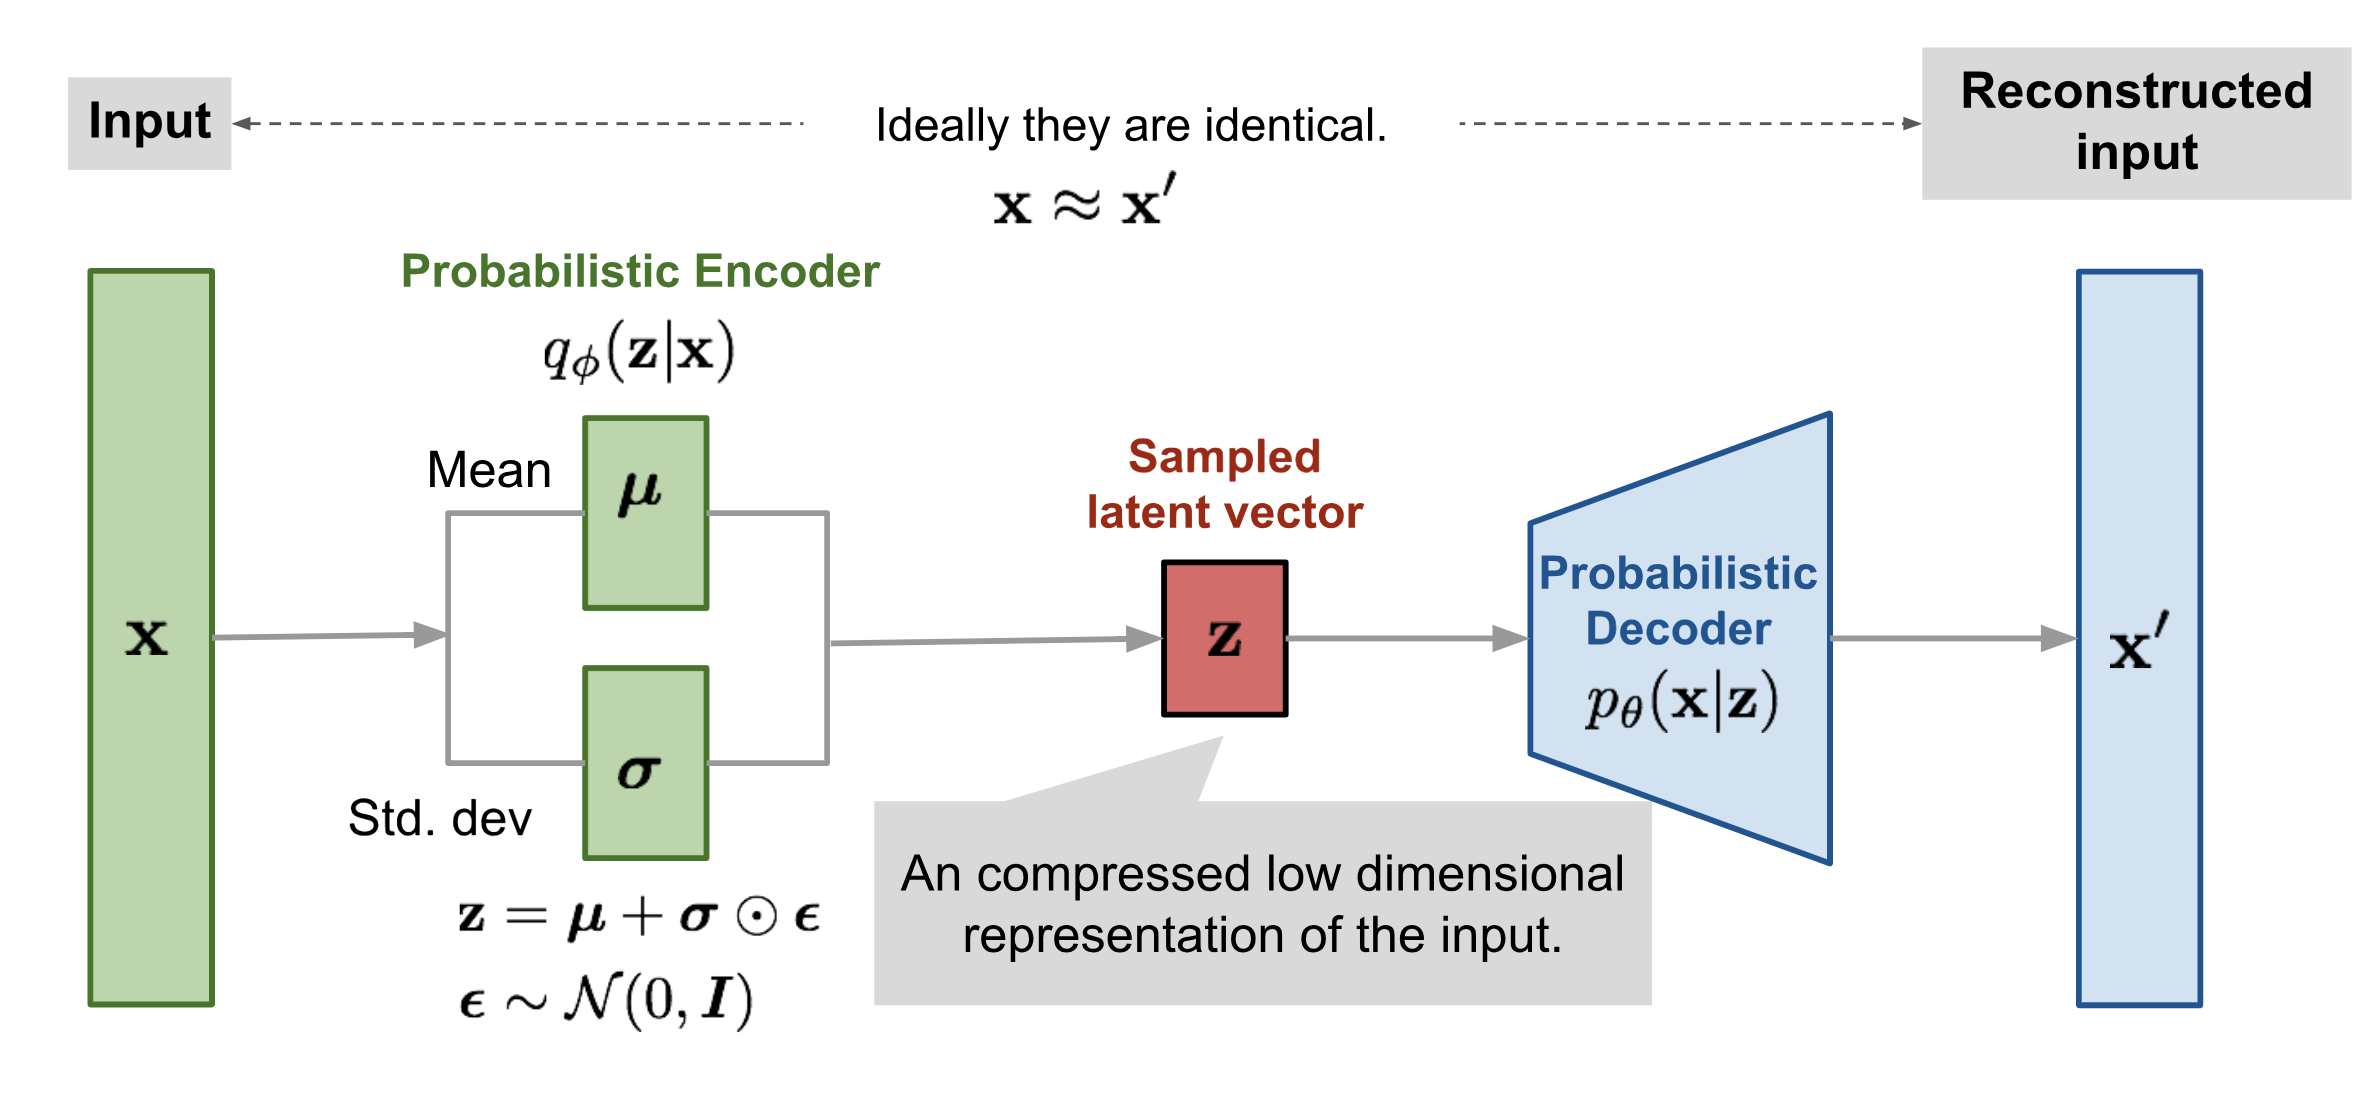
\includegraphics[width=0.8\textwidth]{vae}
\end{center}

\end{frame}

\begin{frame}{Theory of the VAE}

\begin{center}
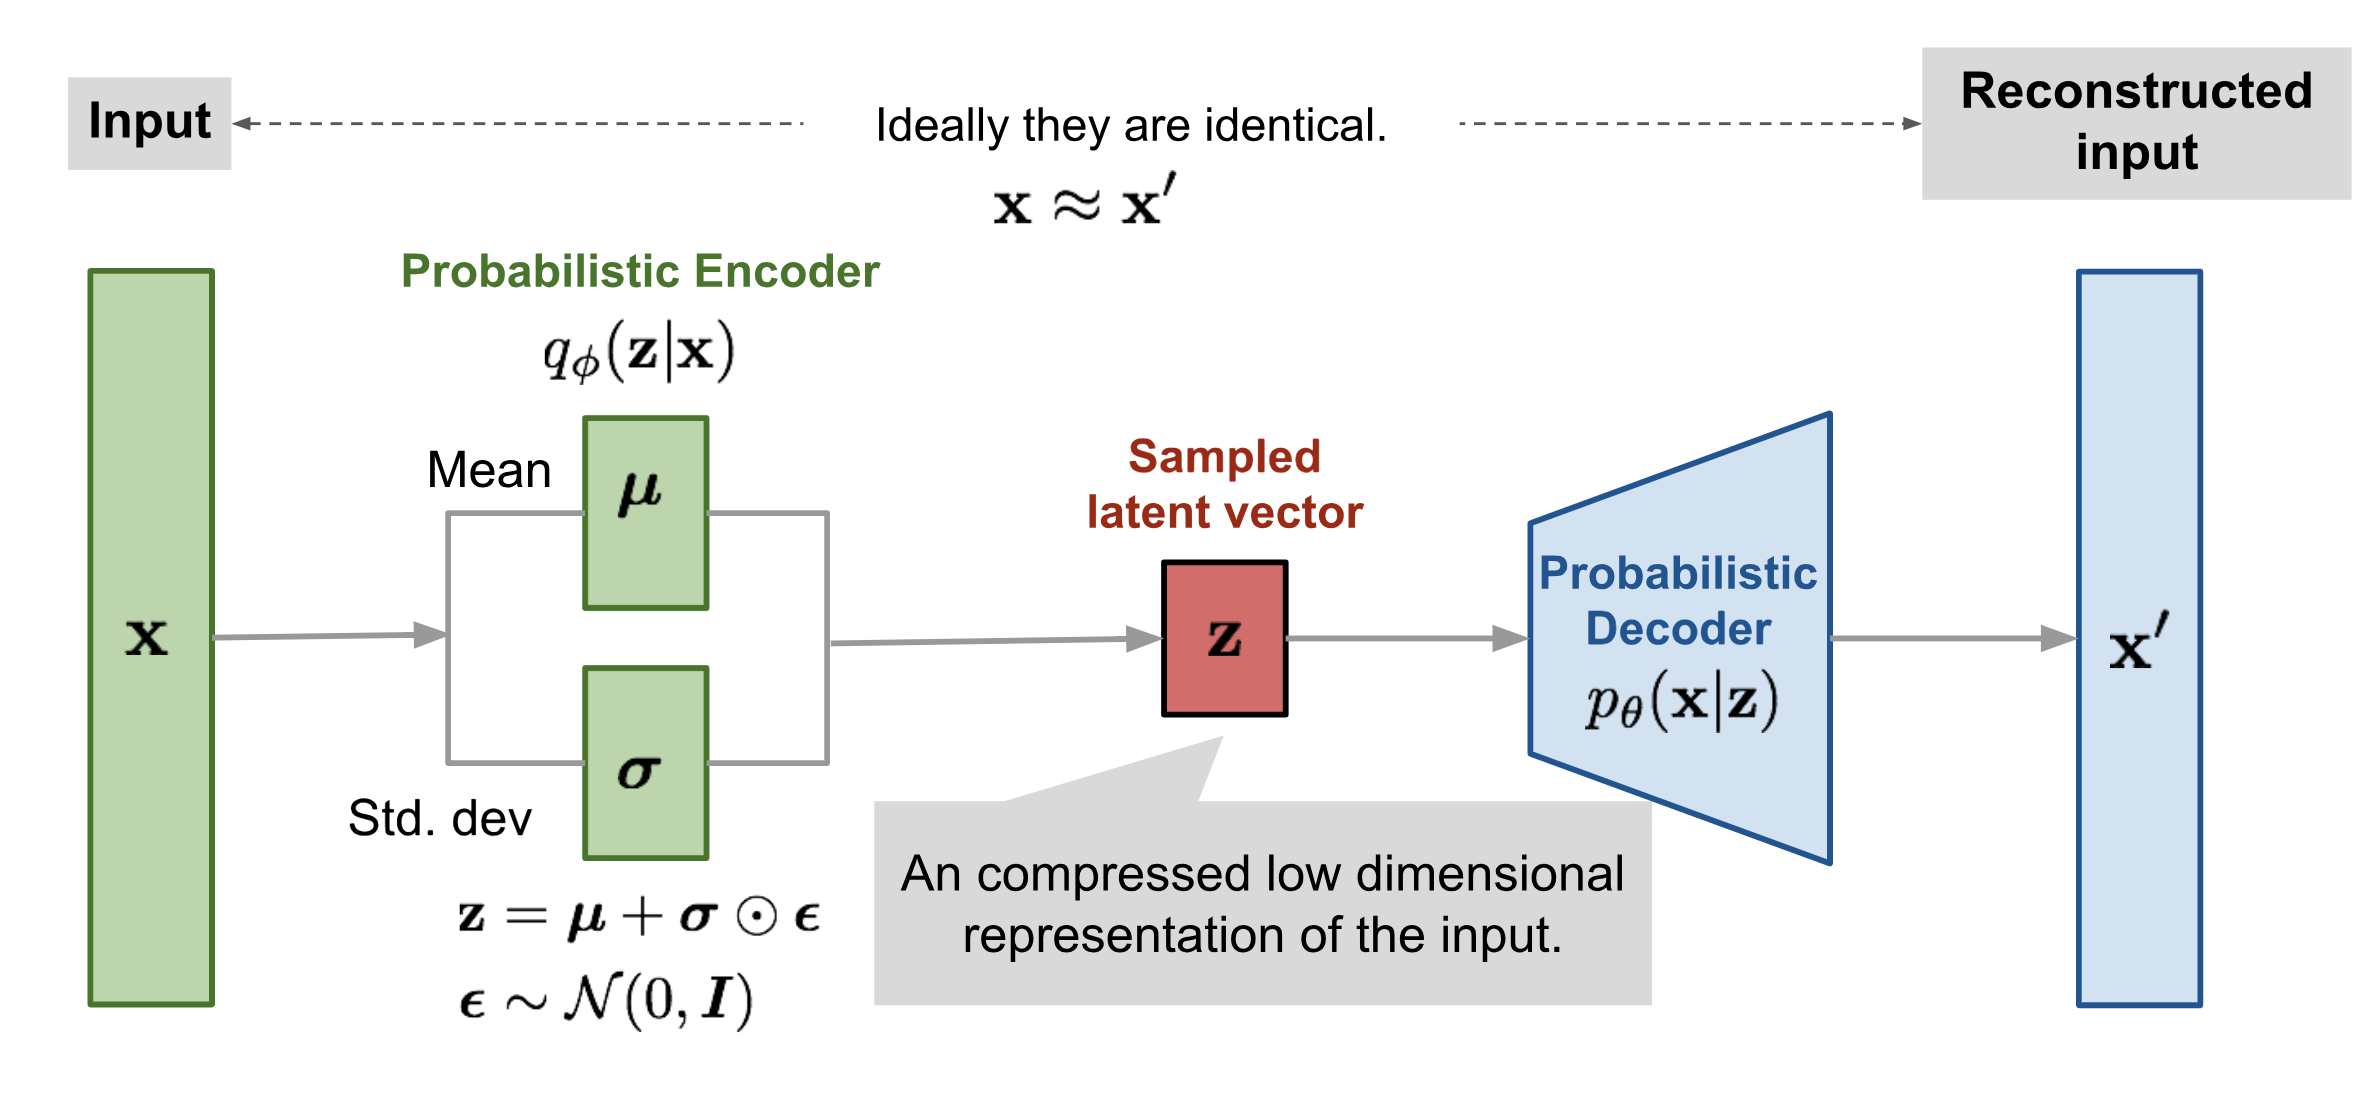
\includegraphics[width=0.8\textwidth]{vae}
\end{center}

\end{frame}

\begin{frame}{Monte-Carlo Markov Chain (MCMC)}

\begin{itemize}

\item MCMC algorithms were originally developed in the 1940’s by physicists at
Los Alamos

\item They were interested in modeling the probabilistic behavior of collections of
atomic particles

\item Simulation was difficult – the normalization constant $Z$ was not known

\item The term “Monte-Carlo” was coined at Los Alamos.

\item Ulam and Metropolis overcame this problem by constructing a Markov chain
for which the desired distribution was the stationary distribution

\item Introduced to statistics and generalized with the Metropolis-Hastings
algorithm (1970) and the Gibbs sampler of Geman and Geman (1984).
\end{itemize}

\end{frame}



\begin{frame}{Markov Chains}

For a state space $\Omega$ s.t. $\mathbf{x}_t\in \Omega$. $\mathbf{x}_t$ is a Markov process if:\\
\vspace{0.1in}
\begin{equation*}
P(\mathbf{x}_{t}|\mathbf{x}_{t-1},\mathbf{x}_{t-2},...,\mathbf{x}_{t-N}) = P(\mathbf{x}_{t}|\mathbf{x}_{t-1})
\end{equation*}
\\
\vspace{0.1in}
which is commonly called the \emph{memoryless property}.\\
\vspace{0.1in}

\begin{itemize}
\item $\mathbf{x}_{t}$ can be generally be $N$-dimensional
\item The chain is called \emph{homogeneous} if $T(\mathbf{x}_{t}|\mathbf{x}_{t-1})$ is time-invariant.
\item For discrete $\Omega$, $T$ is a matrix of probabilities with $T_{ij} = \mathrm{Pr}(i\rightarrow j)$
\item For continuous $\Omega$, $T$ is the joint probability density $T(x_{t},x_{t-1})$
\end{itemize}

\end{frame}

\begin{frame}{Markov Chains}

The Chapman-Kolmogorov equation marginalizes $T(x_{t},x_{t-1})$:

\begin{align*}
P(\mathbf{x}_t) &= \int T(x_{t},x_{t-1})d\mathbf{x}_{t-1}\\
&= \int T(x_{t}|x_{t-1})P(\mathbf{x}_{t-1})d\mathbf{x}_{t-1}
\end{align*} 

The chain satisfies \emph{detailed balance} if 
 
\begin{equation*}
T(x_{t},x_{t-1})P(x_{t}) = T(x_{t-1},x_{t})P(x_{t-1})
\end{equation*}

\vspace{0.1in}
which guarantees there is a unique stationary distribution $P_{0}(x_{t})$  

\end{frame}

\begin{frame}{Monte-Carlo Markov Chain (MCMC)}

A stationary distribution satisfies

\begin{equation*}
P_{0}(\mathbf{x}_t) = \int T(x_{t}|x_{t-1})P_{0}(\mathbf{x}_{t-1})d\mathbf{x}_{t-1}
\end{equation*} 

\begin{itemize}
\item If a process is Markov e.g., Brownian motion, Ornstein-Uhlenbeck, $P_{0}(x_{t})$ is a solution to the SDE 
\item We can also design $T(x_{t},x_{t-1})$ s.t. $P_{0}(x_{t})$ is a distribution we cannot sample from easily such as the Ising model
\item The notion of ``time" in the second case is artificial
\item There are several MCMC algorithms, we will focus on Gibbs MCMC
\end{itemize}

\end{frame}

\begin{frame}{Gibbs sampling}

\begin{itemize}
\item Suppose $p(\mathbf{x})$ is a p.d.f.\ or p.m.f.\ that is difficult to sample from directly.  
\item Suppose, though, that we \textit{can} easily sample from the conditional distributions e.g., $p(x_{1}|x_{2},...,x_{n})$. 
\item  The Gibbs sampler proceeds as follows: 
\begin{enumerate}
\item set $\mathbf{x}$ to some initial starting values
\item then sample $x_{1}|x_{2},...,x_{n}$, then sample $x_{2}|x_{1},...,x_{n}$, and so on.
\end{enumerate}
\end{itemize}
\end{frame}

\begin{frame}{Gibbs sampling}
\begin{enumerate}
\item[0.] Set \textcolor{blue}{$(x_0,y_0)$} to some starting value.
\item[1.] Sample $x_1\sim p(x|y_0)$, that is, from the conditional distribution $X\mid Y=y_0$. \\
\textcolor{blue}{Current state: $(x_1, y_0)$}\\
          Sample $y_1\sim p(y|x_1)$, that is, from the conditional distribution $Y\mid X=x_1$.\\
    \textcolor{blue}{      Current state: $(x_1, y_1)$}\\
\item[2.] Sample $x_2\sim p(x|y_1)$, that is, from the conditional distribution $X\mid Y=y_1$. \\
    \textcolor{blue}{      Current state: $(x_2, y_1)$}\\
          Sample $y_2\sim p(y|x_2)$, that is, from the conditional distribution $Y\mid X=x_2$. \\
            \textcolor{blue}{      Current state: $(x_2, y_2)$}\\
        $\vdots$
\end{enumerate}
Repeat iterations 1 and 2, M times. 
\end{frame}

\section{Probabilistic Graphical Models}

\begin{frame}{Bayesian inference using Gibbs sampling}

Joint distributions factor according to 

\begin{equation*}
P(\mathbf{x})=P(x_{1}|x_{2},...,x_{n})P(x_{2}|x_{3},...,x_{n}),...,P(x_{n})
\end{equation*}

$P(x_{1}|x_{2},...,x_{n})$ may not include all $n-1$ variables

\begin{center}
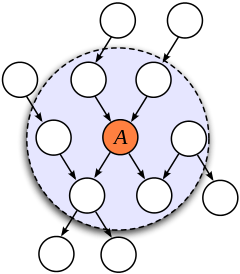
\includegraphics[width=0.4\textwidth]{blanket}
\end{center}

The useful information is called a \textcolor{red}{Markov blanket}

\vspace{0.1in}


\end{frame}

\begin{frame}{Learning graph structure}

Learning the graph structure $\mathcal{G}=(V,E)$ is a common task in machine learning.\\

\end{frame}

\begin{frame}{Applying deep generative models to biological data}
\begin{figure}
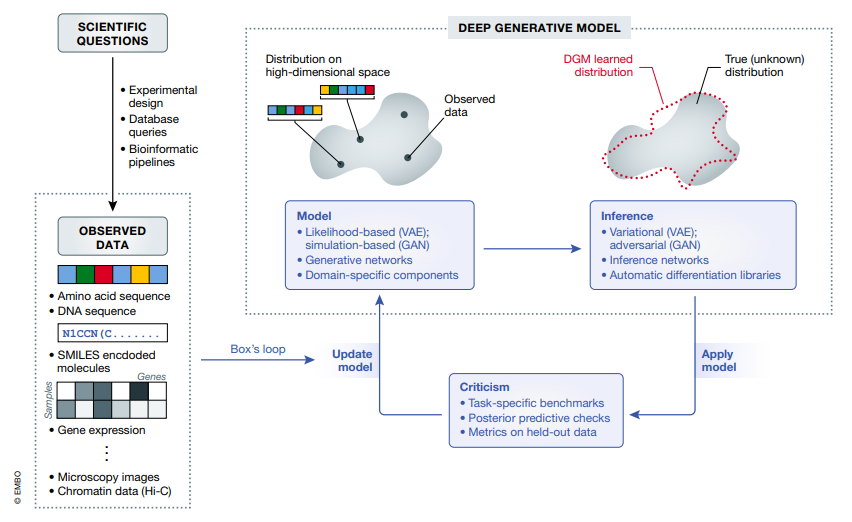
\includegraphics[height=65mm, width=105mm]{dbm}
\end{figure}
\end{frame}

\begin{frame}{Cool biological applications of VAEs}

Sequencing, Imaging, Other stuff

\end{frame}

\section{References}

% Adding the option 'allowframebreaks' allows the contents of the slide to be expanded in more than one slide.
\begin{frame}[allowframebreaks]{References}
	\tiny\bibliography{references}
	\bibliographystyle{apalike}
\end{frame}

\end{document}